\section{GUI}
\subsection{Hauptmenü}
Dies ist die erste Ansicht die der Nutzer zu sehen bekommt. Hier kann er das
Spiel starten und zu freigeschalteten Karten gelangen.

\subsection{Das Spiel}

Das Spiel wird in drei Hauptbereiche unterteilt. Diese werden in eigenen
Abschnitten genauer erläutert. 
\begin{enumerate}[A.]
  \item Kontrollleiste
  \item Sequenzleiste
  \item Karte
\end{enumerate}
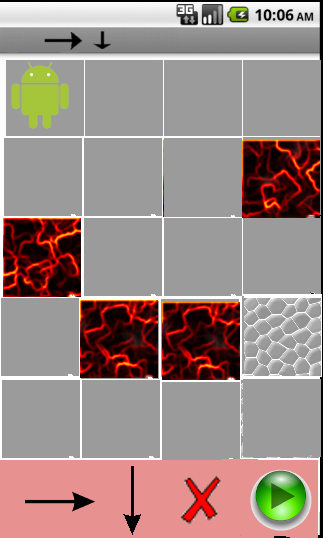
\includegraphics{mockup_game.png}


\subsection{Kontrollleiste}
Die Kontrollleiste enthält die Steuerungselemente.
\begin{enumerate}
  \item Pfeil nach Unten. Beim anklicken wird dieser Pfeil an das Ende der
        Sequenz hinzugefügt.
  \item Pfeil nach Rechts. Bis auf die Richtung identisch mit Pfeil nach Unten.
  \item Start Button. Startet die Sequenz, außer die Sequenz ist nicht valide.
  \item Löschen Button. Löscht die letzte Aktion aus der Sequenz, falls vorhanden.
\end{enumerate}

\subsection{Sequenzleiste}
Die Sequenzleiste zeigt den Aufbau der aktuellen Sequenz an. Wir unterscheiden
zwischen einem aktiven und inaktiven Zustand.

Im aktiven Zustand wird der Fortschritt der Sequenz dargestellt, dazu wird die
laufende Aktion farblich hervorgehoben. In der Zeit kann der Nutzer keine
Änderungen an der Sequenz durchführen.

%\begin{enumerate}
%  \item eingestell
%\end{enumerate}

\subsection{Karte}
Die Karte stellt den Sequenzablauf und die Spielfigur dar. Dieser Bereich ist
verschiebbar, da die Matrix bei steigerung des Schwierigkeitsgrades größer wird.
Die Matrix besteht aus:
\begin{itemize}
  \item Freien Feldern. Diese können von der Spielfigur betreten werden.
  \item Blockierten Feldern / Minen. Sobald die Spielfigur betritt, wird der
        Sequenzablauf beendet.
  \item Endfeldern, wie freie Felder. Werden zusätzlich farblich hervorgehoben,
        um dem Nutzer deutlich zu machen, dass diese Felder erreicht werden
        müssen.
\end{itemize}

Auch bei der Karte unterscheiden wir zwischen aktiven und inaktiven Zuständen.

Der inaktive Zustand dient dem Nutzer als Übersicht. Hier kann er die Matrix
frei verschieben um seine Sequenz planen zu können.
Im aktiven Zustand wird der Ablauf der Sequenz dargestellt, die Matrix wird
automatisch verschoben und der User kann diese nicht mehr selbst verschoeben.


\section{Spielablauf}
Der Nutzer stellt eine Sequenz ein. Diese wird von dem Roboter auf dem
Spielfeld abgelaufen. Sobald die letzte Aktion in der Kette ausgeführt wurde,
springt der Zeiger zurück zur ersten Aktion in der Sequenz. Also wird diese
bis zum Erfolg oder Scheitern wiederholt.

Die Spielfigur wird immer zentriert auf dem Bildschirm dargestellt, also muss
die Matrix bei Bewegungen entsprechend verschoben werden.

Die Mindestanzahl von Aktionen muss eingehalten werden. Ansonsten ist die
Sequenz nicht valide. Die Mindestlänge steigert sich mit dem
Schwierigkeitsgrad.

\includegraphics[width=\dimexpr\textwidth-2\tabcolsep-2pt\relax]{run_sequence.pdf}


\subsection{Spielfortschritt}
Bei erfolgreicher Beendung einer Karte (Level), wird dem Spieler ein Dialog
angezeigt, dass ihm die Wahl ermöglicht zum nächsten Level zu gelangen oder
auf der derzeitigen Karte zu bleiben um seine Lösung noch mal anzusehen.
Dabei wird im Hintergrund der Fortschritt des Spielers gespeichert, da an der
Stelle bereits die nächste Karte freigeschaltet werden soll.
